%% This is file `DEMO-TUDaReport-de.tex' version 3.40 (2024-07-01),
%% it is part of
%% TUDa-CI -- Corporate Design for TU Darmstadt
%% ----------------------------------------------------------------------------
%%
%%  Copyright (C) 2018--2024 by Marei Peischl <marei@peitex.de>
%%
%% ============================================================================
%% This work may be distributed and/or modified under the
%% conditions of the LaTeX Project Public License, either version 1.3c
%% of this license or (at your option) any later version.
%% The latest version of this license is in
%% http://www.latex-project.org/lppl.txt
%% and version 1.3c or later is part of all distributions of LaTeX
%% version 2008/05/04 or later.
%%
%% This work has the LPPL maintenance status `maintained'.
%%
%% The Current Maintainers of this work are
%%   Marei Peischl <tuda-ci@peitex.de>
%%
%% The development respository can be found at
%% https://github.com/tudace/tuda_latex_templates
%% Please use the issue tracker for feedback!
%%
%% If you need a compiled version of this document, have a look at
%% http://mirror.ctan.org/macros/latex/contrib/tuda-ci/doc
%% or at the documentation directory of this package (if installed)
%% <path to your LaTeX distribution>/doc/latex/tuda-ci
%% ============================================================================
%%
% !TeX program = lualatex
%%

\documentclass[
	german,
	accentcolor=9c,% Farbe für Hervorhebungen auf Basis der Deklarationen in den
	type=intern,
	marginpar=false
	]{tudapub}

\usepackage[german]{babel}
\usepackage[autostyle]{csquotes}
\usepackage{graphicx}               % Required for inserting images
\usepackage{amsmath}                % Required for equations
\usepackage{booktabs}                % Required for tables
\usepackage{url}
\usepackage{hyperref}
\usepackage{xcolor}

\usepackage{siunitx}
\usepackage[version=4]{mhchem}

%%%%%%%%%%%%%%%%%%%%%%%%%%%%%%%%%%%%%%%%%%
% Uncomment to change font
%\usepackage{lmodern}
%\renewcommand{\familydefault}{\sfdefault}
%%%%%%%%%%%%%%%%%%%%%%%%%%%%%%%%%%%%%%%%%%

\linespread{1.6}

%Formatierungen für Beispiele in diesem Dokument. Im Allgemeinen nicht notwendig!
\let\file\texttt
\let\code\texttt
\let\pck\textsf
\let\cls\textsf

\begin{document}

\title{Titel}
\author{Autor}
%\date{} % Ohne Angabe wird automatisch das heutige Datum eingefügt

\maketitle

\tableofcontents

\newpage

\section{Aufgabenbeschreibung}
In dieser Aufgabe schreiben Sie einen LaTeX-Bericht unter Verwendung der offiziellen TU-Vorlage über Ihre Datenanalyse des Spotify-Datensatzes. 

\begin{itemize}
\item Keine Sorge: Sie müssen keinen ausführlichen Text über Musiktheorie schreiben. Ihre Antworten können kurz und prägnant sein, solange sie die Fragen vollständig beantworten. Ihr Bericht wird technisch bewertet, wobei der Fokus darauf liegt, ob er die grundlegenden Regeln des wissenschaftlichen Schreibens einhält (siehe Abschnitt \ref{marking_guide}). 

\item Diese Richtlinien sind unten als Tutorial zusammengefasst und dienen auch als initiale LaTeX-Vorlage. Bitte lesen Sie diese sorgfältig und untersuchen Sie die im Rohdokument verwendeten Befehle (links auf dem Bildschirm sichtbar).

\item Ihr endgültiger Bericht sollte keinen Text aus dieser Vorlage enthalten. Ersetzen Sie stattdessen alle Platzhalterinhalte durch Ihre Lösungen der Aufgaben, so wie es in einem echten Laborbericht der Fall wäre. Sie können gerne Abschnitte, Unterabschnitte und andere strukturelle Elemente verwenden, solange sie logisch sind und zur Klarheit und Organisation Ihres Berichts beitragen.
\end{itemize}


\subsection{Richtlinien}       % Starten Sie einen neuen Unterabschnitt innerhalb des Abschnitts

\subsubsection{Gleichungen}  % Starten Sie einen neuen Unterunterabschnitt

Gleichungen sollten mit \LaTeX\,\href{https://www.overleaf.com/learn/latex/Learn_LaTeX_in_30_minutes#Adding_math_to_LaTeX}{\textcolor{blue}{(Link zum Tutorial)}} formatiert werden.

\paragraph{Formatierung von nicht-mathematischem Text}         % Starten Sie einen neuen Absatz
Einige mathematische Funktionen – wie trigonometrische Funktionen, logarithmische Funktionen und Exponentialfunktionen – werden als Textoperatoren und nicht als einfache Variablen behandelt. Diese Funktionen sind in LaTeX vordefiniert und müssen korrekt formatiert werden, um sie von gewöhnlichen Variablen oder Symbolen zu unterscheiden. Ohne den Backslash interpretiert LaTeX diese als Variablen und formatiert sie standardmäßig kursiv. Dies kann mathematische Ausdrücke schwerer lesbar machen und Verwirrung stiften (Tabelle \ref{tab:functions}).

Manchmal muss normaler Text im Mathematikmodus erscheinen, wie z.\,B. Einheiten oder spezifische Bezeichnungen. Verwenden Sie in solchen Fällen \texttt{mathrm}, um aufrechten Text sicherzustellen. Mit \texttt{mathrm} wird sichergestellt, dass nicht-mathematischer Text, wie Einheiten oder Bezeichnungen, im korrekten typografischen Stil erscheint. \emph{Tipp: Eine automatisierte und konsistentere Möglichkeit zur Formatierung von Zahlen und Einheiten finden Sie in der Datei \texttt{siunitx-template}.}

\begin{table}[h!]
\centering
\begin{tabular}{lll}
\toprule
    &    Syntax & Darstellung \\
\midrule
Korrekt & \verb|f(x) = \sin(x) + \ln(x) + \exp(x)| & $ f(x) = \sin(x) + \ln(x) + \exp(x) $  \\
Falsch & \verb|f(x) = sin(x) + ln(x) + exp(x)| & $ f(x) = sin(x) + ln(x) + exp(x) $  \\
\midrule
Korrekt & \verb|v = 5 \, \mathrm{m/s}| & $ v = 5 \, \mathrm{m/s} $  \\
Falsch & \verb|v = 5 \, m/s| & $ v = 5 \, m/s $  \\
\bottomrule
\end{tabular}
\caption{LaTeX-Mathematiksyntax und Darstellung von mathematischem und nicht-mathematischem Text.}
\label{tab:functions}
\end{table}

Wie in Gleichung \eqref{eq:reaction} gezeigt, können (und sollten) Gleichungen ebenfalls beschriftet und im Haupttext referenziert werden. Siehe die Verwendung der Befehle \texttt{label} und \texttt{ref} in diesem Text.

\begin{equation}
\mathrm{A + B \longrightarrow C + D}
\label{eq:reaction}
\end{equation}

\subsubsection{Tabellen}  % Starten Sie einen neuen Unterunterabschnitt

Tabellen sollten verwendet werden, wenn Daten nicht klar im Fließtext dargestellt werden können, wenn viele Zahlen präsentiert werden müssen oder wenn sinnvollere Zusammenhänge durch das tabellarische Format vermittelt werden können. Tabellen sollten den Text und die Abbildungen ergänzen, jedoch keine Informationen duplizieren.

\begin{itemize}  
\item Tabellen sollten einfach und prägnant sein, ohne übermäßigen Gebrauch von horizontalen und insbesondere vertikalen Linien.
\item Alle Tabellen sollten beschriftet sein. Siehe die Verwendung des Befehls \texttt{label} in Tabelle \ref{tab:functions}.
\item Alle Tabellen sollten explizit im Haupttext referenziert werden. Siehe die Verwendung des Befehls \texttt{ref} in diesem Text.
\item Alle Tabellen sollten mit Beschriftungen versehen sein. Beschriftungen sollten eigenständig und informativ sein, sodass sie unabhängig vom Haupttext verständlich sind.
\end{itemize}

\subsubsection{Abbildungen}  % Starten Sie einen neuen Unterunterabschnitt

\begin{itemize}                     
\item Abbildungen sollten eine angemessene Größe und ein passendes Seitenverhältnis aufweisen. Alle Abbildungen im Bericht sollten einheitlich formatiert sein. 
Als allgemeine Richtlinie sollte der Text in einer Abbildung in der Größe mit dem Text im Hauptteil des Dokuments vergleichbar sein. Sie können eine Abbildung in Ihrem Jupyter-Notebook neu plotten, bis Sie mit ihrem Seitenverhältnis und ihrer Schriftgröße zufrieden sind. Experimentieren Sie mit \texttt{width}, um die Abbildung in Relation zur Seitenbreite zu skalieren \href{https://www.overleaf.com/learn/latex/Inserting_Images#Changing_the_image_size_and_rotating_the_picture}{(siehe, wie es in Abbildung \ref{fig:bad} und \ref{fig:good} gemacht wurde, und werfen Sie einen Blick in das \textcolor{blue}{Tutorial})}. \emph{Willkommen in der echten Welt des wissenschaftlichen Schreibens.} Tipp: Sobald Sie die für Sie besten Einstellungen identifiziert haben, wenden Sie diese konsequent auf alle nachfolgenden Abbildungen an, um ein einheitliches Erscheinungsbild im gesamten Dokument sicherzustellen.
    \begin{itemize}          
    \item Abbildung \ref{fig:bad} zeigt ein schlechtes Beispiel: Die Abbildung ist unnötig groß. 
    \item Abbildung \ref{fig:good} weist eine angemessene Größe auf, und die Textgröße ist vergleichbar mit dem Haupttext.
    \end{itemize}  
\item Alle Abbildungen sollten beschriftet sein \href{https://www.overleaf.com/learn/latex/Learn_LaTeX_in_30_minutes#Captions,_labels_and_references}{(siehe die Verwendung des Befehls \texttt{label} in Abbildung \ref{fig:bad} und \ref{fig:good}, und werfen Sie einen Blick in das \textcolor{blue}{Tutorial})}.
\item Alle Abbildungen sollten explizit im Haupttext referenziert werden. Siehe die Verwendung des Befehls \texttt{ref} in diesem Text.
\item Alle Abbildungen sollten mit Beschriftungen versehen sein. Beschriftungen sollten eigenständig und informativ sein, sodass sie unabhängig vom Haupttext verständlich sind.
    \begin{itemize}                    
    \item Die Beschriftung der Abbildung \ref{fig:bad} ist nicht informativ. 
    \item Die Beschriftung der Abbildung \ref{fig:good} ist informativ.
    \end{itemize}  
\end{itemize} 

\begin{figure}[htbp]
\centering
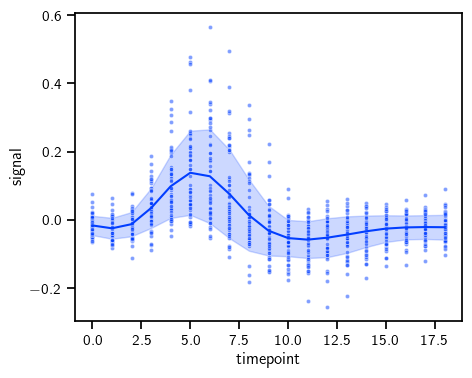
\includegraphics[width=\textwidth]{output.png}
\caption{Signal gegen Zeitpunkt.}
\label{fig:bad}
\end{figure}

\begin{figure}[h]
\centering
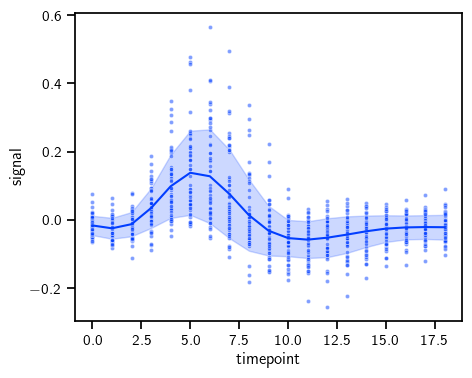
\includegraphics[width=0.6\textwidth]{output.png}
\caption{FMRI-Signale als Funktion der Zeit. Einzelne Datenpunkte werden als Streudiagramm dargestellt. Zu jedem Zeitpunkt werden mehrere Messungen durch ihren Mittelwert (durchgezogene Linie) und die Standardabweichung (schattierter Bereich) zusammengefasst.}
\label{fig:good}
\end{figure}

%\clearpage

\subsubsection{Nützliche Dinge für die Zukunft}  % Starten Sie einen neuen Unterunterabschnitt
\begin{itemize}
\item Sehen Sie sich die Datei \texttt{siunitx-template} an, um zu lernen, wie man Zahlen und deren Einheiten korrekt setzt.
\item \href{https://www.overleaf.com/learn/latex/Chemistry_formulae#Using_mhchem_to_typeset_chemical_formulae_and_equations}{\textcolor{blue}{Setzen chemischer Formeln und Gleichungen}}.
\end{itemize}

\clearpage

\section{Aufgaben}       % Starten Sie einen neuen Abschnitt

\begin{itemize}
\item Lesen Sie alle Richtlinien: Sie enthalten Anweisungen, Hinweise und Hilfestellungen. 
\item Lesen Sie sie erneut.
\item Falls Sie im vorherigen Assignment Kommentare erhalten haben, ist dies der Moment, sie zu berücksichtigen.
\end{itemize}

\subsection{}
\begin{itemize}
\item Beschreiben Sie kurz den Datensatz: Wie viele Spalten hat er?
\item Fügen Sie in Ihrem Notebook den folgenden Code ein und führen Sie ihn aus:
\end{itemize}

\begin{verbatim}
datei = {
    "Kopfzeile": [
        "Title", "Artist", "Year", "Acousticness", "Danceability", 
        "Energy", "Instrumentalness", "Loudness, dB", "Speechiness", 
        "Tempo", "Valence", "Popularity", "Explicit", "Duration, minutes"
    ],
    "Beschreibung": [
        "Der Titel des Songs.", 
        "Der Name des Künstlers oder der Band.",
        "Das Jahr, in dem der Song veröffentlicht wurde.",
        "Ein Wert, der die Wahrscheinlichkeit angibt, dass der Song akustisch ist.",
        "Ein Wert, der beschreibt, wie tanzbar der Song ist.",
        "Ein Wert, der die Intensität und Aktivität des Songs darstellt.",
        "Ein Wert, der den Anteil instrumentaler Inhalte (ohne Gesang) schätzt.",
        "Die durchschnittliche Lautstärke des Songs in Dezibel (dB).",
        "Ein Wert, der den Anteil gesprochener Worte im Song angibt.",
        "Das Tempo des Songs in Schlägen pro Minute (BPM).",
        "Ein Wert, der die Positivität oder 'Fröhlichkeit' des Songs darstellt.",
        "Ein Wert, der die Popularität des Songs basierend auf Streams und Bewertungen angibt.",
        "Ob der Titel explizite Texte enthält oder nicht.",
        "Die Dauer des Songs in Minuten."
    ]
}

kopfzeilen = pd.DataFrame(datei)

print(kopfzeilen.to_latex(index=False))
\end{verbatim}

\begin{itemize}
\item Kopieren Sie die LaTeX-Ausgabe in dieses Dokument und führen Sie sie aus, um das formatierte Ergebnis anzuzeigen. Fügen Sie eine Beschriftung und eine Legende zur Tabelle hinzu. Beschreiben Sie die Tabelle kurz in einem Satz und verweisen Sie dabei korrekt auf ihre Beschriftung.
\end{itemize}

\subsection{}
\begin{itemize}
\item Fügen Sie die Grafik ein, die Sie in Aufgabe 5 erstellt haben.
\item Stellen Sie sicher, dass die Grafik korrekt beschriftet und mit einer Legende versehen ist. Fügen Sie eine kurze Beschreibung hinzu, die korrekt darauf verweist.
\item Welche Art von Fehlerbalken wird in dieser Grafik angezeigt? Identifizieren Sie die verwendete Formel und fügen Sie sie in das Dokument ein. Achten Sie dabei auf die korrekte Formatierung für nicht-mathematischen Text.
\end{itemize}

\subsection{}
\begin{itemize}
\item Fügen Sie die Diagramme ein, die Sie in Aufgabe 6 erstellt haben, und zwar als zwei separate Abbildungen.
\item Stellen Sie sicher, dass die Abbildungen korrekt beschriftet und mit Legenden versehen sind. Fügen Sie eine kurze Beschreibung hinzu, die korrekt darauf verweist und den Schiefe-Wert angibt.
\end{itemize}

\subsection{}
\begin{itemize}
\item Fügen Sie das Heatmap-Diagramm ein, das Sie in Aufgabe 7 erstellt haben. 
\item Stellen Sie sicher, dass die Grafik korrekt beschriftet und mit einer Legende versehen ist. Fügen Sie eine kurze Beschreibung hinzu, die korrekt darauf verweist und Ihre Entscheidung rechtfertigt, in der nächsten Aufgabe Loudness vs.\,Energy zu plotten.
\end{itemize}

\subsection{}
\begin{itemize}
\item Fügen Sie die Kurvenanpassung ein, die Sie in Aufgabe 8.3 erstellt haben. 
\item Stellen Sie sicher, dass die Grafik korrekt beschriftet und mit einer Legende versehen ist. Fügen Sie eine kurze Beschreibung hinzu, die korrekt darauf verweist, sowie die Gleichung, die Sie für die Anpassung verwendet haben. Die Gleichung sollte korrekt formatiert sein und den Textoperator $\log$ berücksichtigen.
\end{itemize}

\subsection{}
\begin{itemize}
\item Fügen Sie die Diagramme ein, die Sie in Aufgabe 9 erstellt haben, und zwar als zwei separate Abbildungen. 
\item Stellen Sie sicher, dass die Abbildungen korrekt beschriftet und mit Legenden versehen sind. Fügen Sie eine kurze Beschreibung hinzu, die korrekt darauf verweist und den Schiefe-Wert angibt.
\item Welche Art von Fehlerbalken wird im Balkendiagramm angezeigt? Identifizieren Sie die verwendete Formel und fügen Sie sie in das Dokument ein. Achten Sie dabei auf die korrekte Formatierung für nicht-mathematischen Text.
\end{itemize}

\subsection{}
\begin{itemize}
\item Fügen Sie die Diagramme ein, die Sie in Aufgabe 10 erstellt haben, und zwar als zwei separate Abbildungen. 
\item Stellen Sie sicher, dass die Abbildungen korrekt beschriftet und mit Legenden versehen sind. Fügen Sie eine kurze Beschreibung hinzu, die korrekt darauf verweist.
\item Erstellen Sie eine Tabelle, in der jede Zeile die Explizit-Werte (Ja und Nein) darstellt. Die Spalten zeigen die durchschnittlichen Popularitätswerte (eine Dezimalstelle) für verschiedene Zeiträume: Insgesamt, Seit 1980, Seit 1990, Seit 2000 und Seit 2010.
\end{itemize}

\section{Bewertungskriterien}\label{marking_guide}
Insgesamt sind 17 Punkte verfügbar: Sie benötigen mindestens 12 Punkte zum Bestehen.
Ihre Aufgaben werden anhand der folgenden technischen Kriterien bewertet:
\begin{enumerate}
\item Haben die Abbildungen eine angemessene Größe und ein korrektes Seitenverhältnis, einschließlich Schriftgröße?
\item Werden die Abbildungen korrekt im Text referenziert?
\item Sind die Abbildungslegenden informativ und eigenständig verständlich?
\item Werden die Tabellen korrekt im Text referenziert?
\item Sind die Tabellenlegenden informativ und eigenständig verständlich?
\item Sind die Gleichungen korrekt formatiert?
\item Werden die Gleichungen korrekt im Text referenziert?
\end{enumerate}

\small
\begin{tabular}{cccccccccccc}
\toprule
 & Fig 1 & Fig 1 & Fig 1 & Fig 2 & Fig 2 & Fig 2 & Table & Table & Equation & Equation \\
  & Aesthetics & Reference & Caption & Aesthetics & Reference & Caption & Caption & Reference & Formatting & Reference \\
\midrule
Task 1 & - & - & - & - & - & - & 0.5 & 0.5 & - & - \\
Task 2 & 0.3 & 0.5 & 0.5 & - & - & - & - & - & 0.5 & 0.5 \\
Task 3 & 0.3 & 0.5 & 0.5 & 0.3 & 0.5 & 0.5 & - & - & - & - \\
Task 4 & 0.3 & 0.5 & 0.5 & - & - & - & - & - & - & - \\
Task 5 & 0.3 & 0.5 & 0.5 & - & - & - & - & - & 0.5 & 0.5 \\
Task 6 & 0.3 & 0.5 & 0.5 & 0.3 & 0.5 & 0.5 & - & - & 0.5 & 0.5 \\
Task 7 & 0.3 & 0.5 & 0.5 & 0.3 & 0.5 & 0.5 & 0.5 & 0.5 & - & - \\
\bottomrule
\end{tabular}

\end{document}
